\documentclass[letterpaper]{physor2024}

%%% Packages Required by Class (already included)
% fancyhdr
% lastpage
% titling
% titlesec
% ragged2e
% enumitem
% amsmath
% graphicx
% geometry
% newtxtext
% newtxmath
% hyperref
% cleveref
% caption
% authblk
% apptools
% appendix
% ifpdf
% epstopdf

%%% Some other useful packages
% \usepackage{tikz}
% \usepackage{color}
% \usepackage{subcaption}
% \usepackage{algcompatible}
% \usepackage{bm}
% \usepackage{array}

% GLOSSARIES
\usepackage[acronym,nomain,nonumberlist,nogroupskip,nopostdot]{glossaries} % for glossary of acronyms
\setacronymstyle{long-short}
\loadglsentries{glossary}
\makeglossaries
% \renewcommand*{\glstextformat}[1]{\textcolor{black}{#1}} % make glossary color black

% % This file contains custom commands that Lewis uses frequently in LaTeX documents

\usepackage{subcaption}
\usepackage{hyperref}
\hypersetup{colorlinks,allcolors=black}
% % for more https://tex.stackexchange.com/questions/88400/hyperref-changing-the-linkcolor-locally-in-the-toc

% custom equation commands
\newcommand{\QOR}{\qquad \text{OR} \qquad}
\newcommand{\QAND}{\qquad \text{AND} \qquad}
\newcommand{\QTHUS}{\qquad \text{THUS} \qquad}
\newcommand{\QWITH}{\qquad \text{WITH} \qquad}
\newcommand{\QFOR}{\qquad \text{FOR} \qquad}
\newcommand{\QSO}{\qquad \text{SO} \qquad}
\newcommand{\QWHERE}{\qquad \text{WHERE} \qquad}
\newcommand{\QWHEN}{\qquad \text{WHEN} \qquad}
\newcommand{\LINE}{\par\noindent\rule{\textwidth}{0.4pt}\par}
\newcommand{\toinf}{\rightarrow\infty}
\newcommand{\tozero}{\rightarrow0}
\newcommand{\qeq}{\overset{?}{=}}
\newcommand{\ceq}{\overset{\checkmark}{=}}
\newcommand{\Poi}{\text{Poisson}}
\newcommand{\keff}{$k_{e\!f\!f}$}
\newcommand{\kinf}{$k_{\!i\!n\!f}$}
\renewcommand{\epsilon}{\varepsilon} % squiggly epsilon

\def\brac#1{\{#1\}}
\def\Brac#1{\big\{#1\big\}}
\def\BRAC#1{\bigg\{#1\bigg\}}
\def\angbrac#1{\langle#1\rangle}
\def\Angbrac#1{\big\langle#1\big\rangle}
\def\ANGBRAC#1{\bigg\langle#1\bigg\rangle}
\usepackage{float}
\usepackage{multirow} % for special table
% % SI Units
\usepackage{siunitx}
\DeclareSIUnit\n{n}
\DeclareSIUnit\sp{sp}
\title{OpenMC Depletion Analysis of the Virtual Test Bed Gas-Cooled Microreactor}
% \title{Title of the Paper Goes Here: Capitalize the First Letter of Major Words, Centered, 14-Point Times New Roman, on the Second Line from the Top Margin, Not More Than Three Lines Long}

%%% Authors (use arabic numbers: 1, 2, 3, etc. for affiliationNumber)
%%% \addAuthor{GivenName MiddleInitial. FamilyName}{affiliationNumber}
\addAuthor[ligross@wissc.edu]{Lewis I. Gross}{1}
\addAuthor{Paul P.~H. Wilson}{1}
\addAuthor{Benjamin Lindley}{1}

%%% Affiliations (from authblk)
%%% \addAffiliation{affiliationNumber}{Name of Institute, City, State/Country}
\addAffiliation{1}{University of Wisconsin - Madison, Madison, Wisconsin}

%%% Write text for abstract
%%% Most text modifying commands will work in abstract
\Abstract{OpenMC is a state-of-the art, \gls{os} Monte Carlo transport code. This work uses OpenMC for depletion analysis of an infinite-assembly model of the \gls{vtb} \gls{gcmr}. This microreactor is prismatic, \gls{triso}-fueled, and helium gas-cooled. Since the \gls{gcmr} is intended for load-following, a depletion analysis was run at 100\%, 50\%, and 10\% of the rated power (225 kWt) for both explicitly represented \gls{triso} and volume-homogenized fuel. The time steps used were twice as long and ten times as long for the lower power cases, respectively, to ensure the same total burnup occurred at each time step. The isotopics after one year of operation at steady-state were compared at each power between both fidelities.}

%%% List up to 5 keywords separated by a comma
\keywords{OpenMC, TRISO, depletion, microreactor, gas-cooled}

%%% Provide a short title for the header on odd pages
\shortTitle{Depletion of a TRISO Fueled, Gas-Cooled Microreactor }

%%% Provide a short author listing for the header on even pages
\authorHead{Gross and Wilson}

%%% If LaTeX reports the line number of an error at \begin{document} it
%%%   is most likely due to an error in one of the commands above
\begin{document}

\section{INTRODUCTION}\label{sec:intro}
For advanced reactors, especially those early in the design stage, sufficient \gls{ms} is required to ensure the success of the design concept. The \gls{vtb} \cite{vtb2023} is a repository of reactor models used for research and demonstration of current tools in the nuclear industry as a part of the \gls{neams} initiative. Various types of reactors are available on the \gls{vtb}. Microreactors are one viable class of next generation systems with ongoing efforts to model them using \gls{neams} tools \cite{Stauff-preliminary-applications-2021, Stauff-applications-2022}. One key advantage of microreactors is the ability to supply power to lower demand areas that may not be able to consume power on the order of a GW reactor or to areas needing temporary power, e.g.~natural disaster relief efforts. While microreactors can be very diverse in fuel, coolant, and general design, there is interest in combining \gls{htgr} and microreactor technologies. \glspl{htgr} have the benefits of higher electricity conversion efficiency due to the high temperature coolant and the desirable melting properties of \gls{triso} fuel. Adding these benefits to a microreactor bring many attractive features together. Previous work on the \gls{vtb} \gls{gcmr} includes analysis of the system for a two day load-following transient \cite{Abdelhameed-ANS-2022}. This work coupled Griffin \cite{GRIFFIN}, BISON \cite{BISON}, and SAM \cite{SAM} using the \gls{moose} framework. \textbf{add more?} Griffin is a deterministic transport solver that was used for neutronics. BISON is a fuel performance code that can compute heat conduction in the solid parts of thesystem. SAM is a system analysis code that was used for 1-D fluid flow of the coolant channels. While previous works used Griffin for neutron transport, this work chose OpenMC as an alternative to Griffin due to the \gls{os} status of the software, as well to take advantage of Monte Carlo and depletion capabilities in OpenMC.

% While this work looks to extend models of the GCMR, the software selected for this and future analyses will be OpenMC for neutron transport, \gls{moose}'s \gls{hcm} for heat conduction, and \gls{thm} for 1-D



% M&S -> VTB -> MICROREACTORS -> GCMR -> previous GCMR work

\section{DEPLETION THEORY}\label{sec:depletion}
Tracking the isotopic composition of nuclear reactors is a highly important task, as nuclide number density directly influences the solution of the transport equation. Isotopes exposed to neutron flux will transmute into radioisotopes that have various modes of decay, creating new isotopes that did not exist at the start of operation, as well as decaying into other isotopes already in the system. The rate at which isotopes transmute and decay into each other depends on the transport solution via the reaction rates, which depend directly on the neutron flux. This relationship causes the coupling between transport and depletion to behave non-linearly \cite{romano-depletion-2021}.

Certain isotopes have more influence on the system than others. For example, Xenon-135 has an extremely high neutron absorption cross section. It is so high that its negative reactivity insertion influences the positioning of the control elements. Xenon-135 is particularly important in load-following contexts, in which the power changes once or twice per day, as it's concentration increases when power decreases, and it is burned off when power increases again. This matters more in load-following contexts because the Xenon-135 half-life is on the order of 9 hours \cite{d-and-h}. For context, the load following schedule in Abdelhameed et al. has high power for 12 hours, lower power for 7 hours, and 2.5 hour ramps between them \cite{Abdelhameed-ANS-2022}. Considering these rates, the transient behavior for load-following will be more interesting since the power, and neutron flux, changes on a similar timescale as the Xenon-135 half-life.

To model burnup, transmutation and decay cross sections of the isotopes are combined with the computed flux to determine production and destruction rates for each isotope. These formulate a system of differential equations for the nuclide densities. For isotope $i$ with number density $N_{i}(t)$, the Bateman or burnup equations describe the time dependent isotopic composition, given by

\begin{multline} \label{eq:batemen}
    \frac{dN_{i}}{dt} =
    \sum_{j} \bigg[f_{j\rightarrow{i}}\int_{0}^{\infty} \sigma_{j}(E,t)\phi(E,t)dE + \lambda_{j\rightarrow{i}}\bigg]N_{j}(t) \\
    -\bigg[\int_{0}^{\infty} \sigma_{i}(E,t)\phi(E,t)dE
    +\sum_{j}\lambda_{i\rightarrow{j}}\bigg] N_{i}(t),
\end{multline}

\noindent where $\sigma_{j}(E)$ is the transmutation cross section of isotope $j$ at energy $E$, $f_{j\rightarrow{i}}$ is the fraction of transmutation reactions for nuclide $j$ that produce nuclide $i$, and $\lambda_{j\rightarrow{i}}$ are the decay constants for decay modes in nuclide $j$ that produce nuclide $i$. The system of equations for isotopes $i\in[1,n]$ can be expressed in matrix notation using the nuclide vector $\mathbf{n}\in\mathbb{R}^{n}$
\begin{equation} \label{eq:burnup matrix odes}
    \frac{d\textbf{n}}{dt} =
    \textbf{A}(\textbf{n},t) \textbf{n}
    \QWITH
    \textbf{n}(0) = \textbf{n}_{0},
\end{equation}

\noindent where $\textbf{A}\in\mathbb{R}^{n\times n}$ is the burnup matrix. Since the transport equation depends on number density and $\textbf{A}$ depends on the solution to the transport equation, $\textbf{A}$ then also depends on number density. Because ``the timescale over which material compositions change is sufficiently long ... the transport equation can be solved as a steady-state equation" \cite{romano-depletion-2021}. Taking the burnup equations as steady-state allows the earlier non-separable equation to be solved via separation solution
\begin{equation} \label{eq:separable burnup matrix odes}
    \frac{d\textbf{n}}{dt} =
    \textbf{A}(\textbf{n}) \textbf{n}
    \QWITH
    \textbf{n}(0) = \textbf{n}_{0},
\end{equation}

\noindent The solution to which is
\begin{equation} \label{eq:separation solution}
     \textbf{n}(t) = \exp(\textbf{A}t) \textbf{n}_{0}
\end{equation}

\noindent Solving \cref{eq:separable burnup matrix odes} and \cref{eq:separation solution} involves two separate components \cite{romano-depletion-2021}:
\begin{enumerate}
    \item Using a numerical method to integrate the matrix $\textbf{A}$ in \cref{eq:separable burnup matrix odes} forward in time. This usually involves taking one or more matrix exponential.
    \item Evaluating the matrix exponential $\exp(\textbf{A}t)$ or the action of the matrix exponential on a vector of nuclide concentrations.
\end{enumerate}

The key to correctly representing $\textbf{n}(t)$ is to use small enough time steps that $\textbf{A}$ remains \textit{constant enough} to get the new nuclide concentrations, then updating $\textbf{A}$ forward in time to account for the fact that $\textbf{A}$ \textit{does} have time dependence.

\section{SYSTEM DESCRIPTION}\label{sec:system}
The system analyzed is based from the \gls{vtb} \gls{gcmr}. \cref{fig:vtb_gcmr} shows a diagram of the system. The overall structural material of the assembly is graphite with cylindrical holes for various compacts: burnable poison, a central control rod, moderator, coolant, and fuel. The fuel uses 19.95\% enriched Uranium inside the kernel of \gls{triso} particles. The moderator uses YH$_{2}$ encased in a FeCrAl envelope. The poison compacts contain B$_{4}$C burnable absorber spheres. The coolant uses helium and the control rod chamber has a B$_{4}$C rod, where helium fills the space when the control rod is not fully injected; this helium is not circulating like the coolant. There is a top and bottom reflector made of BeO; only the top reflector has space for the control rod \cite{Abdelhameed-ANS-2022}.
\begin{figure}[h]
    \centering
    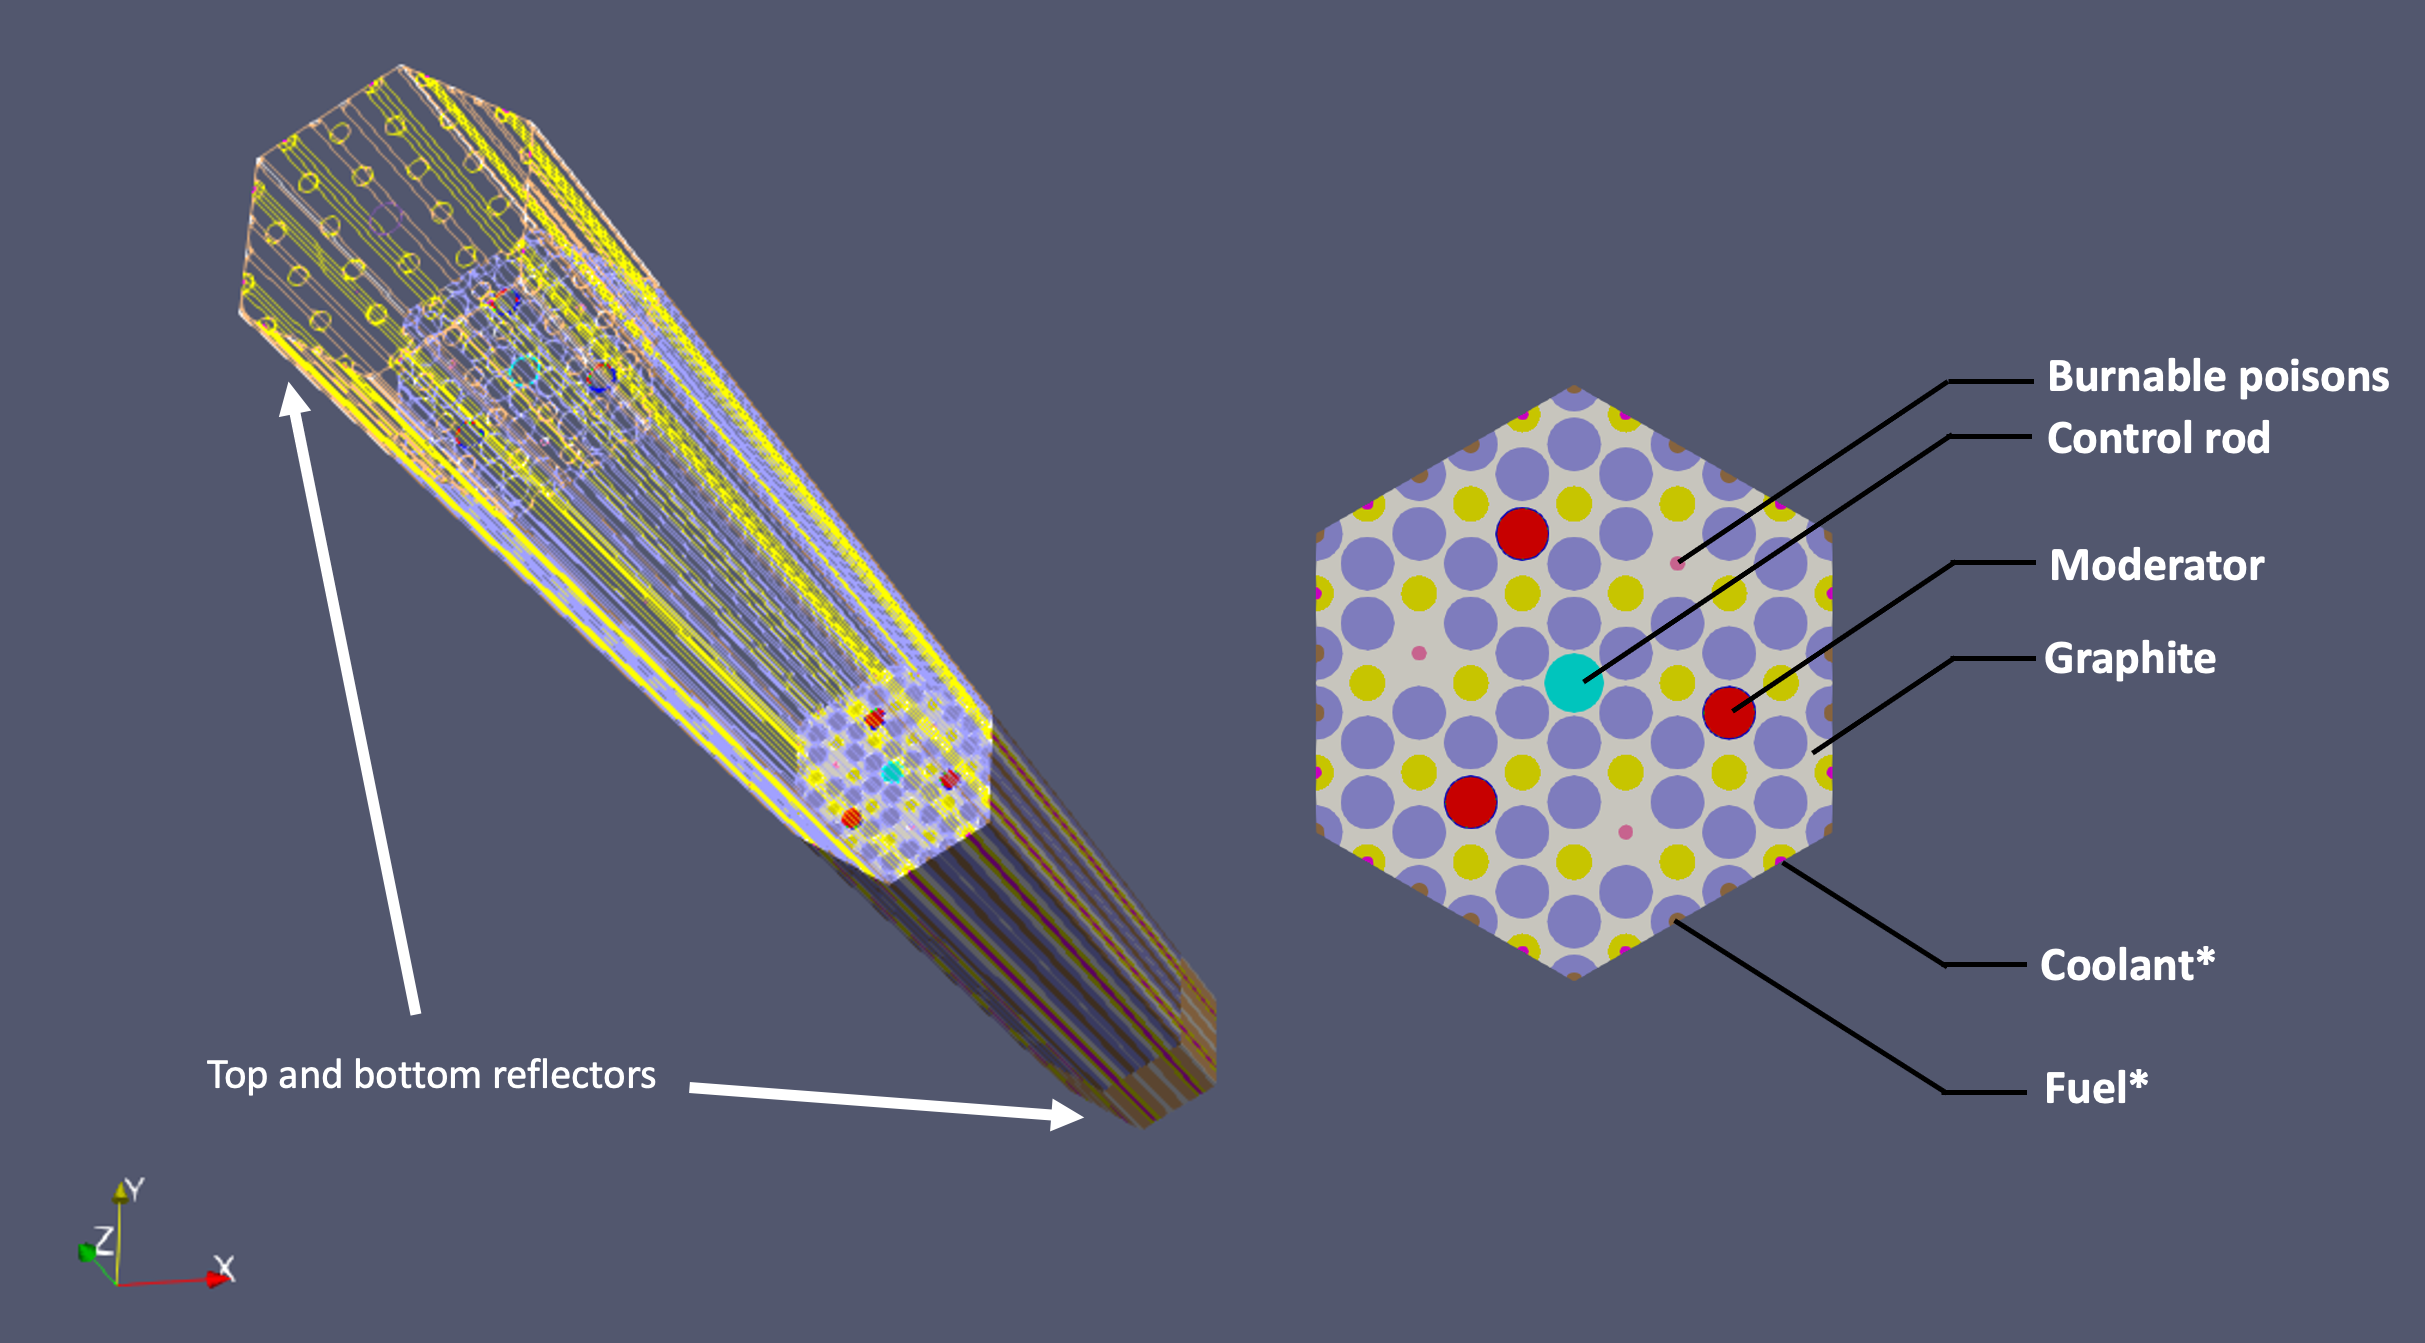
\includegraphics[width=0.75\linewidth]{figures/vtb_gcmr_diagram.jpg}
    \caption{An image of the \gls{vtb} \gls{gcmr} along with a cross section of the fuel containing section of the system.}
    \label{fig:vtb_gcmr}
\end{figure}
\section{OPENMC MODEL}\label{sec:openmc_model}
There are two aspects to the OpenMC model that will each be described. The first is assembling the geometry, material, and tally definitions. In OpenMC, a python script is used to generate XML files that will be used by a neutronics simulation. After that, the depletion simulation settings are defined in a separate script that take the XML files generated and use them to set up everything needed to iterate between transport and depletion steps using the correct time integration method and time steps.
\subsection{Model Definition}\label{sec:model_def}
Describe aspects of gcmr and show some visualizations
\begin{figure}[h!]
    \centering
    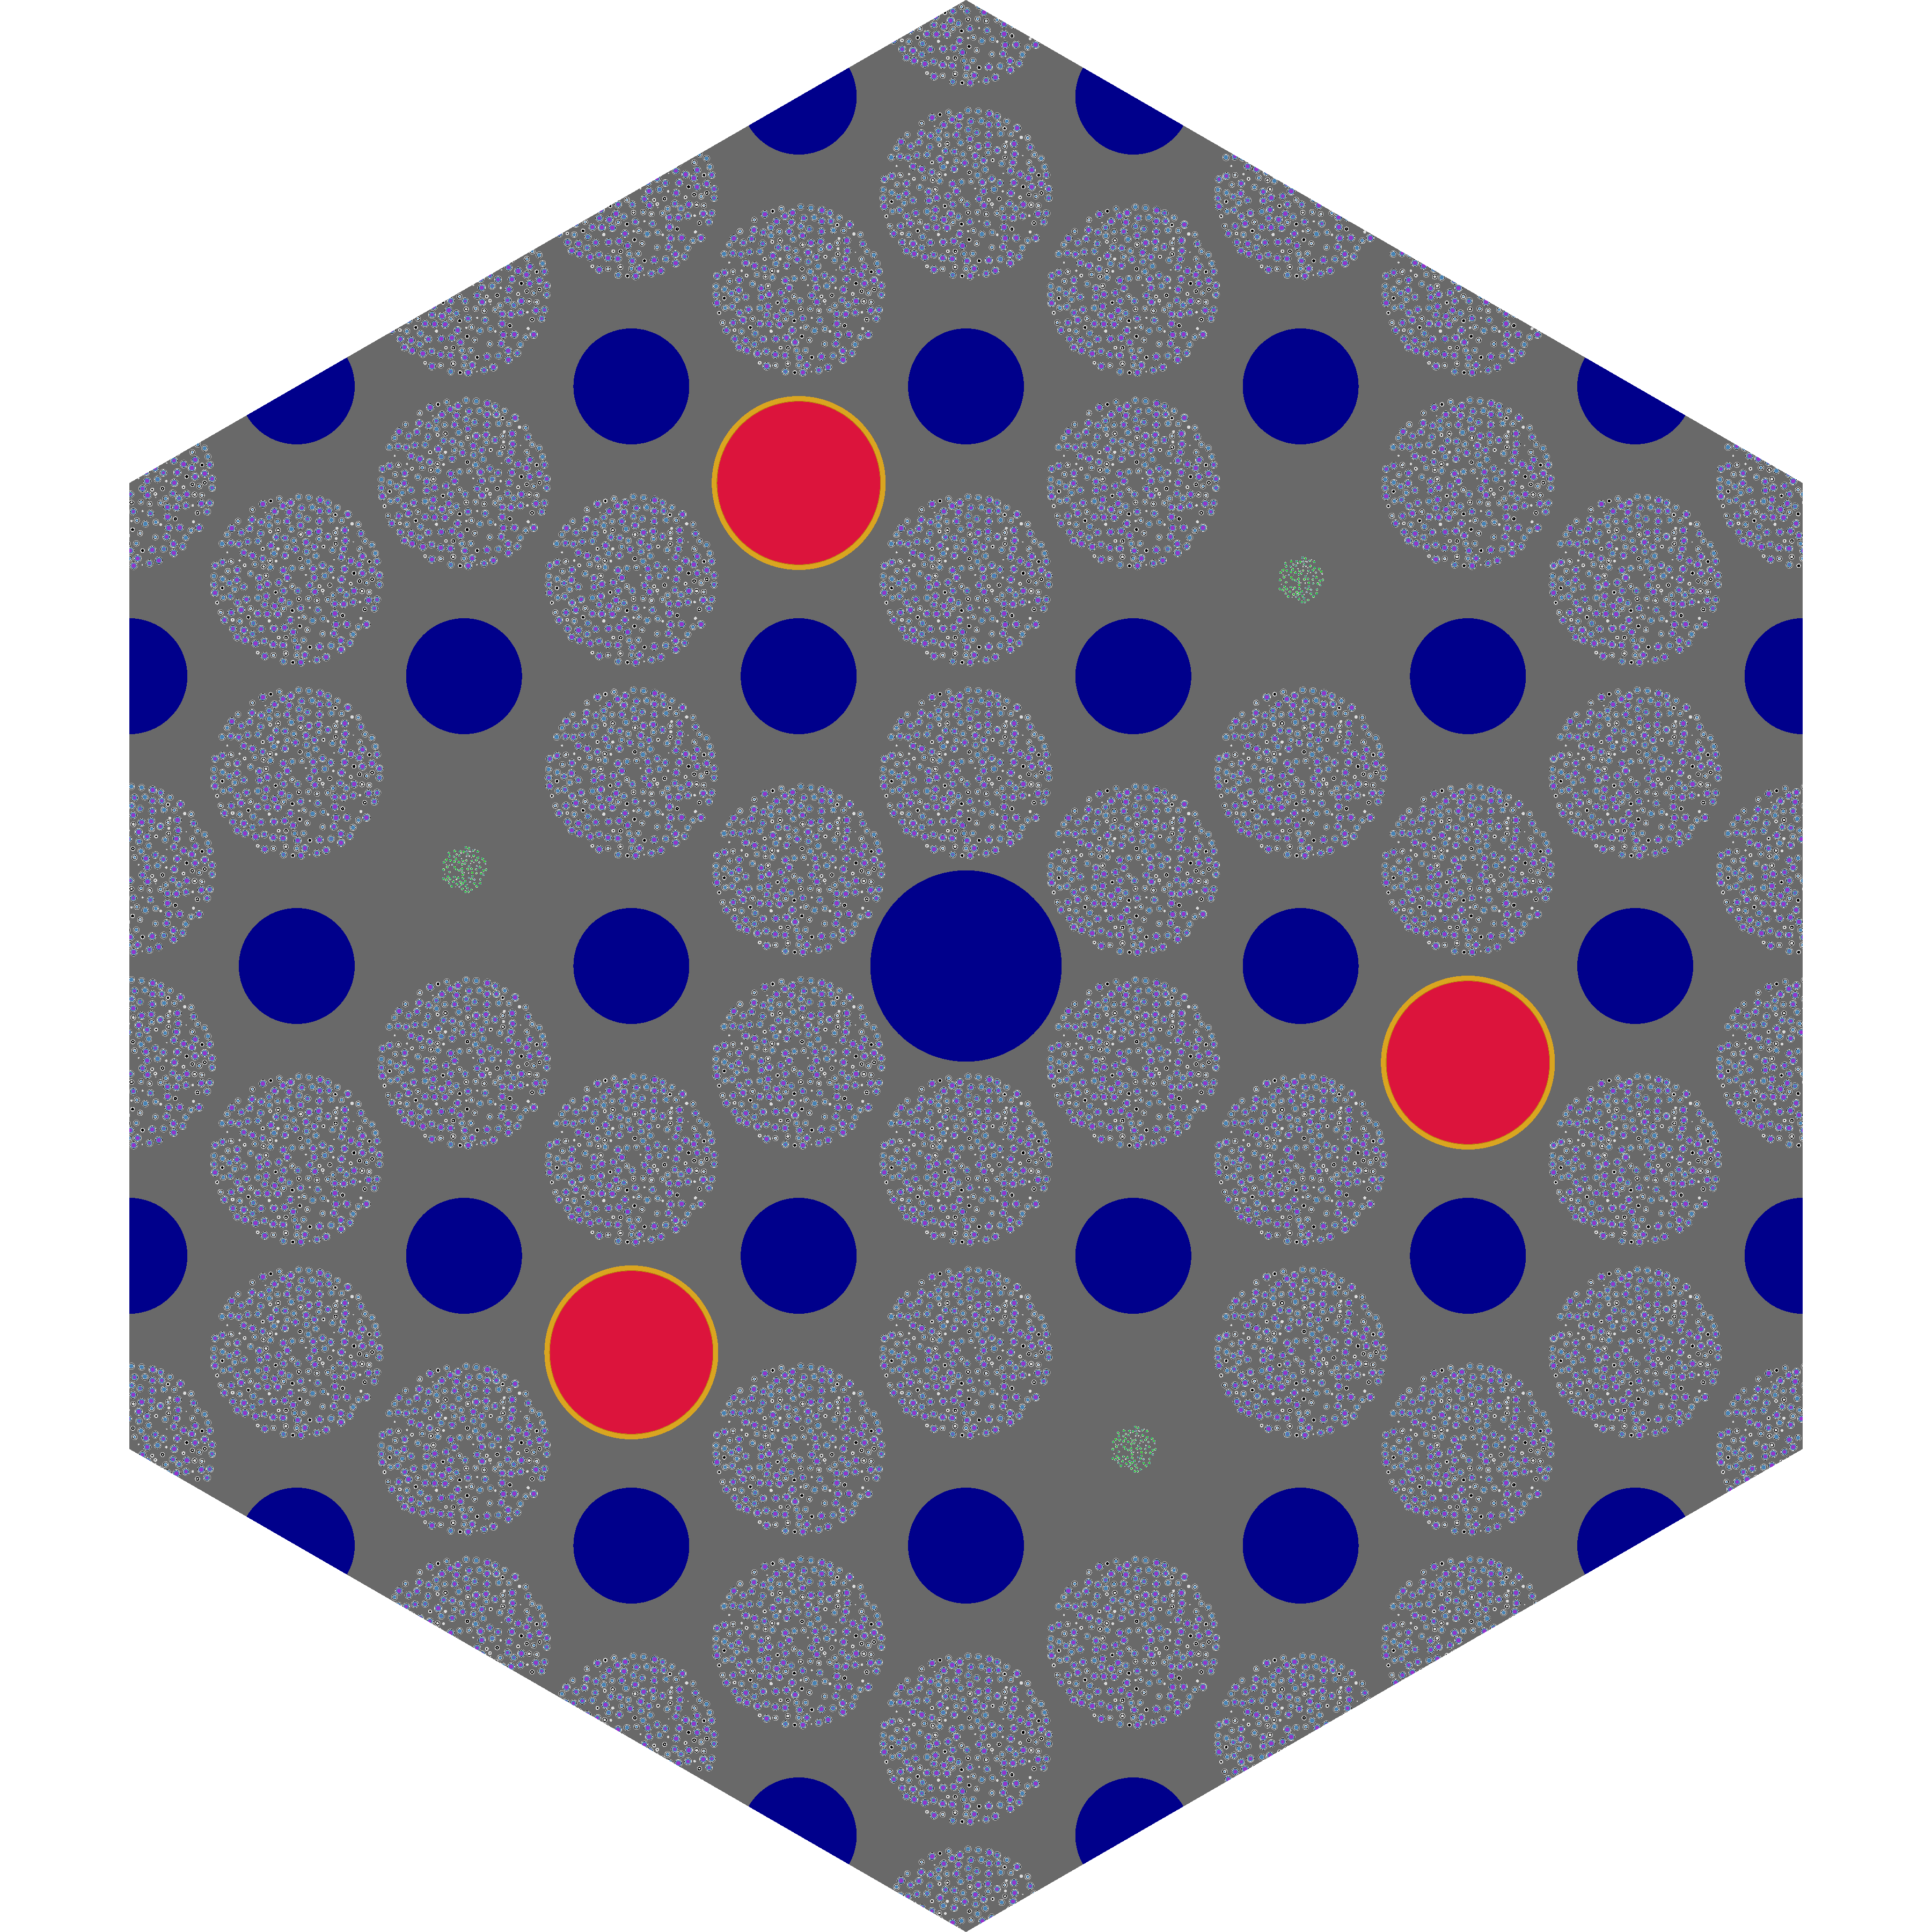
\includegraphics[width=0.55\linewidth]{figures/active_height.png}
    \label{fig:active_slice}
    \caption{A radial slice of the active region. Gray corresponds to graphite in the matrix or pyrolitic carbon, dark blue corresponds to helium coolant, red corresponds to YH$_{2}$ moderator, gold corresponds to FeCrAl, green corresponds to the B$_{4}$C poison particles (packed at 25 percent in graphite), and purple corresponds to the fuel kernel in the \gls{triso} particles (packed at 40 percent in graphite).}
    \label{fig:core_slice_sbs}
\end{figure}
\begin{figure}[h!]
    \centering
    \begin{subfigure}{0.49\linewidth}
        \centering
        
\includegraphics[width=0.75\linewidth]{figures/lower_reflector.png}
        \caption{A slice of the lower reflector, colored by material.}
        \label{fig:lower_reflector_slice}
    \end{subfigure}
    \begin{subfigure}{0.49\linewidth}
        \centering
        
\includegraphics[width=0.75\linewidth]{figures/upper_reflector.png}
        \caption{A slice of the upper reflector, colored by material.}
        \label{fig:upper_reflector_slice}
    \end{subfigure}
    \par\medskip
    \caption{A radial  slice of the lower reflector (left) and the upper reflector (right). The difference between the upper and lower reflectors is that the upper reflector has an extra compact for the B$_{4}$C control rod. Dark blue corresponds to helium coolant
    and light blue corresponds to BeO, while the B$_{4}$C control rod is shown in green.}
    \label{fig:upper_reflector_slice_sbs}
\end{figure}
\subsection{Depletion Simulation Definition}\label{sec:depl_sim}

In this work, the system is held at constant power for each case. This has some implications for the time stepping scheme chosen. To correctly account for the rapid build up of strong neutron absorbers, a few short initial time steps are included to increase those nuclides' accuracy. Since the simulations are constant power, the time steps can be lengthened after this initial transient behavior, after allowing these important isotopes to reach a steady-state.


\section{RESULTS}\label{sec:results}
Various quantities

\begin{figure}[!h]
    \centering
    \begin{subfigure}{0.49\linewidth}
        \centering
        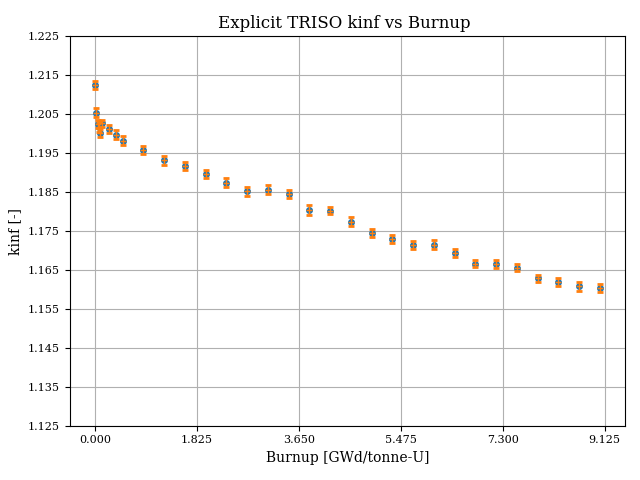
\includegraphics[width=\linewidth]{figures/explicit_kinf_vs_burnup.png}
        \caption{Explicit}
        \label{fig:explicit}
    \end{subfigure}
    \begin{subfigure}{0.49\linewidth}
        \centering
        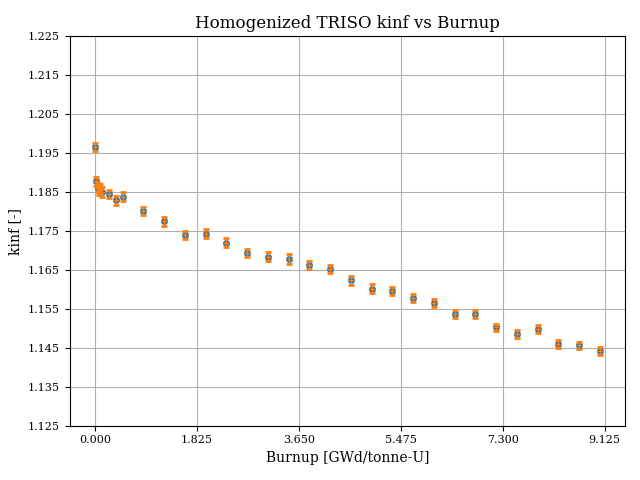
\includegraphics[width=\linewidth]{figures/homogenized_kinf_vs_burnup.png}
        \caption{Homogenized}
        \label{fig:explicit}
    \end{subfigure}
    \caption{Pictured above is results for \kinf both for the explicit \gls{triso} representation and homogenized  }
\end{figure}

\section{CONCLUSIONS}\label{sec:conclusions}
Present summary and conclusions here

Future work: multiphysics Cardinal simulation (OpenMC-MOOSE-THM coupling). Future future work: depletion-multiphysics coupling.

\section*{NOTE TO ORGANIZERS}
Put a note here about what results are planned to be included for the full paper.

\section*{ACKNOWLEDGEMENTS}
The authors would like to thank the OpenMC development team for their guidance in model setup and assistance with software. The first author was supported in part by the US Nuclear Regulatory Commission's Graduate Fellowship Program administered by the University of Wisconsin-Madison.

\printglossaries

\bibliographystyle{physor2024}
\bibliography{physor2024}

\end{document}